\documentclass [a4paper,11pt]{article}

\usepackage [francais]{babel}
\usepackage[utf8]{inputenc}%       encodage du fichier source
\usepackage[T1]{fontenc}%          gestion des accents (pour les pdf)
\usepackage[a4paper]{geometry}%    taille correcte du papier
\usepackage{hyperref}%			   gestion des hyperliens
\usepackage{graphicx}%			   gestion des images
\usepackage{fancyhdr}%
\usepackage{lastpage}%			   pour avoir le numero de page
\usepackage{fancyvrb}%			   meilleur verbatim
\usepackage{chngcntr}%			   pour numéroté les figures au lieux du numéro de section
\usepackage[toc,page]{appendix}%   pour les annexes

% Chemin par defaut des images
\graphicspath{{img/}}

\pagestyle{fancyplain}
\fancyhf{}
\cfoot{\thepage\ sur \pageref{LastPage}}


\begin{document}

\begin{titlepage}
\begin{center}
{\bf Université Sciences et Technologies - Bordeaux1} \vspace{0.5cm}\\

{\bf {\large Master 2 Informatique : Genie logiciel parcours conduite de projet}}\\
%{\emph{Rapport du Projet d'Etude et de Développement }}\\\vspace{1cm}

\begin{figure}[!ht]
  \centering
  
\includegraphics[scale=0.2]{img/uniBx-logo}

  \label{fig:logUniBx}
\end{figure}


{\large{\bf{Rapport:}}}\\\vspace{1cm}
{\huge{\bf Visualisation interactive de topologie de plates-formes parallèles avec lstopo et HTML}}\\\vspace{0.5cm}





\end{center}

\hspace{1cm}\textbf{Réalisé par:} GreenScrum \\
%\bigskip

\hspace{1cm}\textbf{Encadré par:} Philippe Narbel , David Auber.\\


\hspace{1cm}\textbf{Client:} Brice Goglin\\



\end{titlepage}





\tableofcontents

\newpage

\section{Introduction}

\subsection{Présentation du projet}
Le but du projet est de proposer un logiciel de visualisation au format HTML d'une topologie de machines. Cette topologie est constituée d'informations matérielles de chaque machine. Ces données servent à àméliorer les calculs parallèles en optimisant l'utilisation du matériel. Les données à utiliser sont extraites du module lstopo de la bibliothèque logicielle hwloc

\subsection{Réalisation du projet}
Le projet devait être fait en 2 parties avec une partie en C et une partie Web. Le but de la 1ère partie devait être de créer une exportation des données à visualiser. Mais, après discussion avec le client, nous avons compris que ce n'est pas nécessaire. En effet, une exportation au format XML existe déjà, et elle est suffisante pour fournir les données nécessaires à la création de l'application de visualisation.

\newpage
\section{Architecture}

\subsection{MVC}

\subsection{Technologies}

\subsection{Fonctionnalités}
\newpage

\section{Intégration Continue}

Intégration continue est une étape importante à mettre en place dans le processus de développement logiciel. Nous parlerons donc ici de cette pratique et de l'outil utilisé au cours de ce projet.

\begin{center}
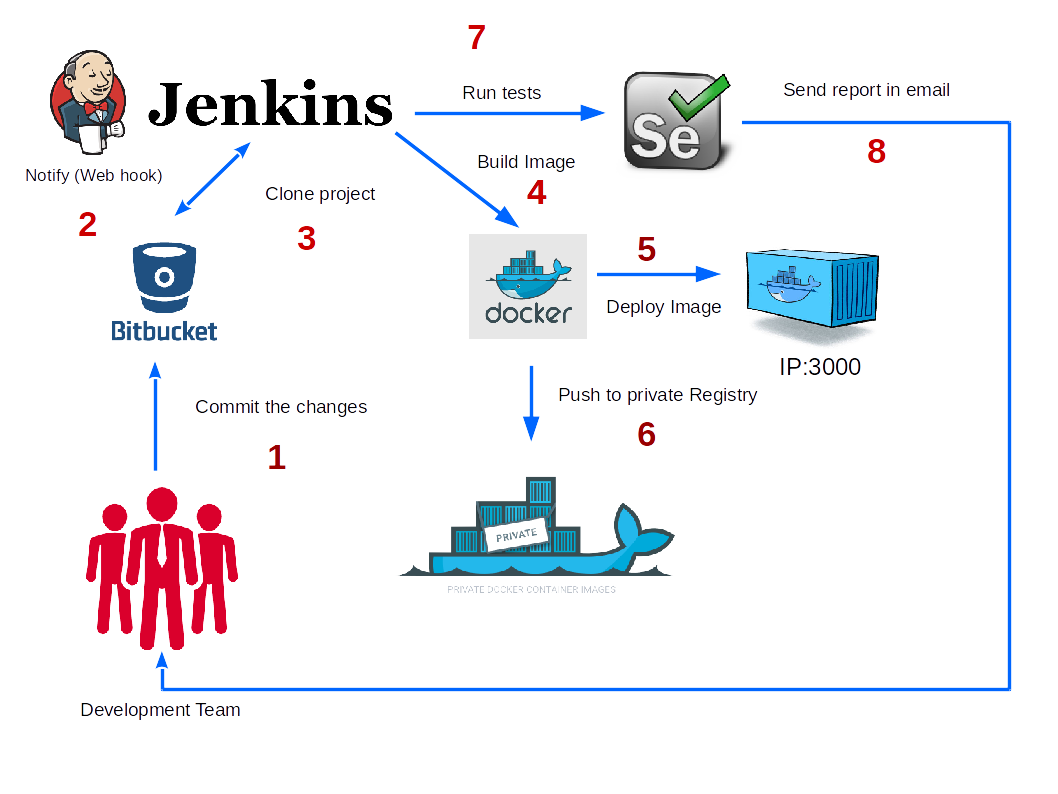
\includegraphics[scale=0.5]{img/ci.png}
\end{center}

Au moment d’un push d’un ou plusieurs commit au niveau de Bitbucket (sur la banche \textbf{release}) on déclenche via un hook la tâche de build qui permet la construction de l'image Docker à partir de Dockerfile, le push de cette image dans un dépot privé, le déploiement de cette image dans un container exposer sur le port 80 et enfin de passage des TUs au niveau de Jenkins. Dès qu’une modification du code est donc poussée sur le repository, il y a vérification que l’ensemble fonctionne toujours.

\begin{center}
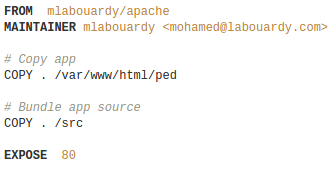
\includegraphics[scale=0.7]{img/Dockerfile.png}
\end{center}

\subsection{Bitbucket}

Un système de versionnement, il a été choisi pour héberger les sources des projets internes et clients. Pour notre projet on a utilisé 3 branches:\newline

\begin{itemize}
 \item \textbf{master} utilisé pour la phase de développement
 \item \textbf{release} utilisé pour la phase de production
 \item \textbf{docs} utilisé pour les documents (rapport, maquettes, cadrage ...)
\end{itemize}

\subsection{Jenkins}

Serveur d'intégration continue, il est capable d’aller se connecter à un outil de gestion de sources (Dans ce cas Git) et de voir si des modifications ont été effectuées. S’il en détecte, il peut lancer un \textbf{build} qui va pouvoir lancer un certain nombre d’actions(déploiement automatisé, tests unitaires ...)

\subsection{Docker}

Docker est un système de container linux ultra léger basé sur les cgroups, lxc et aufs.\newline

L'idée est la suivante pour un build:\newline

\begin{itemize}
 \item Jenkins crée une image docker à partir de Dockerfile
 \item Jenkins push l'image dans un dépot privé
 \item Jenkins crée un container docker à partir de cette image\newline
\end{itemize}
\newline
Les containers sont running de manière continue, permettant ainsi aux responsables du projet et au client de tester la dernière version du produit poussé manuellement à partir de Jenkins.

\subsection{Private Registry}

Depot pour stocker l'ensemble des versions de l'application tout au long de la phase de développement

\begin{center}
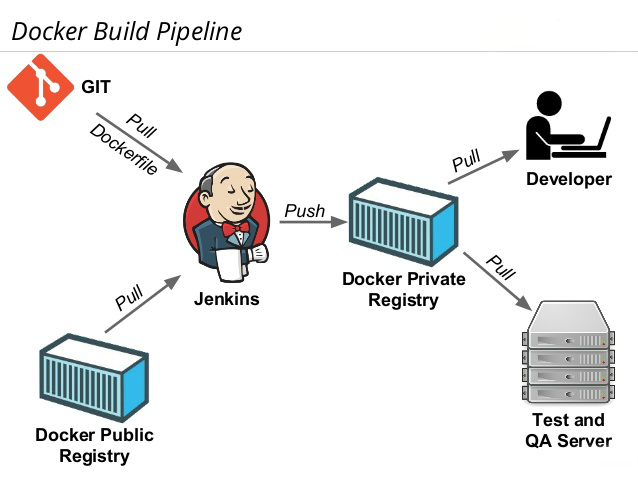
\includegraphics[scale=0.4]{img/registry.png}
\end{center}

L'avatange d'utilisation d'un docker private registry c'est avoir un systéme de versionning pour l'application. et rendre disponible facilement le dernier exécutable.
\subsection{Selenium Webdriver}
WebDriver est un framework de tests fonctionnels issu du projet Selenium, célèbre outil d'automatisation de tests pour navigateurs.\newline

Un exemple des test faites avec l'API Selenium c'est la mesure du temps d'execution pour un ensemble des exemples d'Architecture.

\begin{center}
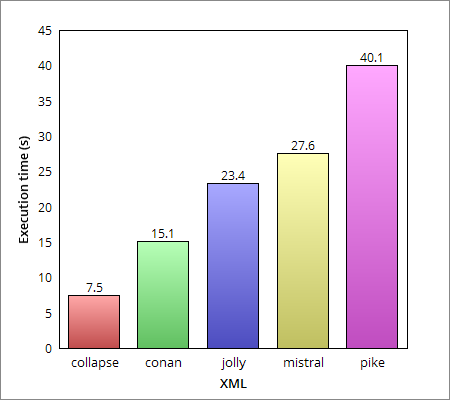
\includegraphics[scale=0.4]{img/benchmark.png}
\end{center}

\subsection{JSLint/CSSLint}

La qualité du code est vitale pour qu'un projet soit pérenne sur le moyen et long terme. De nombreux outils existent pour automatiser les contrôles et générer des rapports statistiques:\newline

\textbf{JSLint} est un analyseur de code Javascript. Son but est de parser le code Javascript pour vérifier que vous respecter les règles de coding Javascript.\newline

\begin{center}
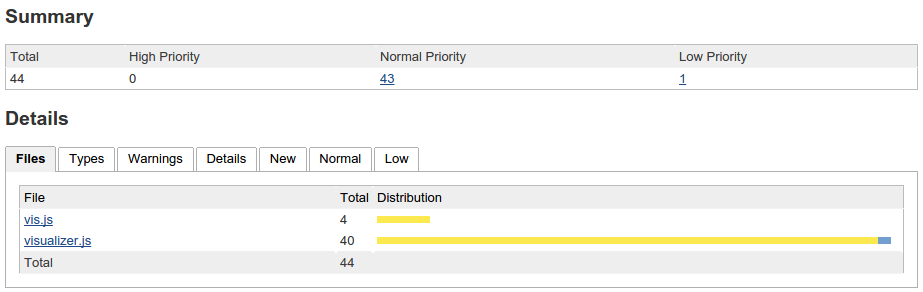
\includegraphics[scale=0.4]{img/checkstyle.png}
\end{center}

\textbf{CSSLint} détecte les problèmes d'une feuille de style CSS.

\begin{center}
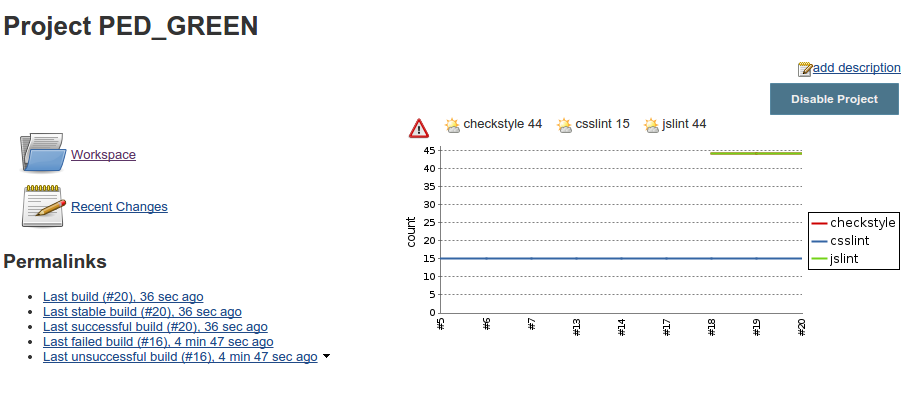
\includegraphics[scale=0.4]{img/jslint.png}
\end{center}

\subsection{AngularJS Batarang}

Afin de développer tester, déboguer et surveiller notre application AngularJS, on a installé un plugin sur le navigateur:\newline

Une extension de Google Chrome. Il permet d'observer le code en action, de faire des benchmarks sur les fonctions, modules, etc...

\newpage
\section{Gestion de projet}

\subsection{Scrum}

\subsection{Outils complémentaires}

\newpage

\newpage

\section{Critiques}

\subsection{Technologies}

\subsection{IceScrum}

\subsection{Performances}

\subsection{Améliorations possibles}

\newpage

\nocite{*}
\bibliographystyle{plain}
\bibliography{report}




\end{document}
